\chapter{Anhang}\label{ch:appendix}

\section{Vollständiger Java-Code für UserRegistry-Beispiel}\label{sec:user-registry-full}

\begin{center}
    \code{User.java}
    \inputminted[breaklines]{java}{chapter/fulib-scenarios/java/User.java}

    \code{UserRegistry.java}
    \inputminted[breaklines]{java}{chapter/fulib-scenarios/java/UserRegistry.java}

    \code{UserRegistryTest.java}
    \inputminted[breaklines]{java}{chapter/fulib-scenarios/java/UserRegistryTest.java}
\end{center}

\section{Scenario-Lexer-Grammatik}\label{sec:scenario-lexer-grammar}

\inputminted[breaklines]{antlr}{chapter/fulib-scenarios/grammars/ScenarioLexer.g4}

\section{Scenario-Parser-Grammatik}\label{sec:scenario-parser-grammar}

\inputminted[breaklines]{antlr}{chapter/fulib-scenarios/grammars/ScenarioParser.g4}

\section{Ergebnisse der Vorlesungsumfrage PM 19/20 zu fulib.org, FulibScenarios und FulibMockups}\label{sec:survey-results}

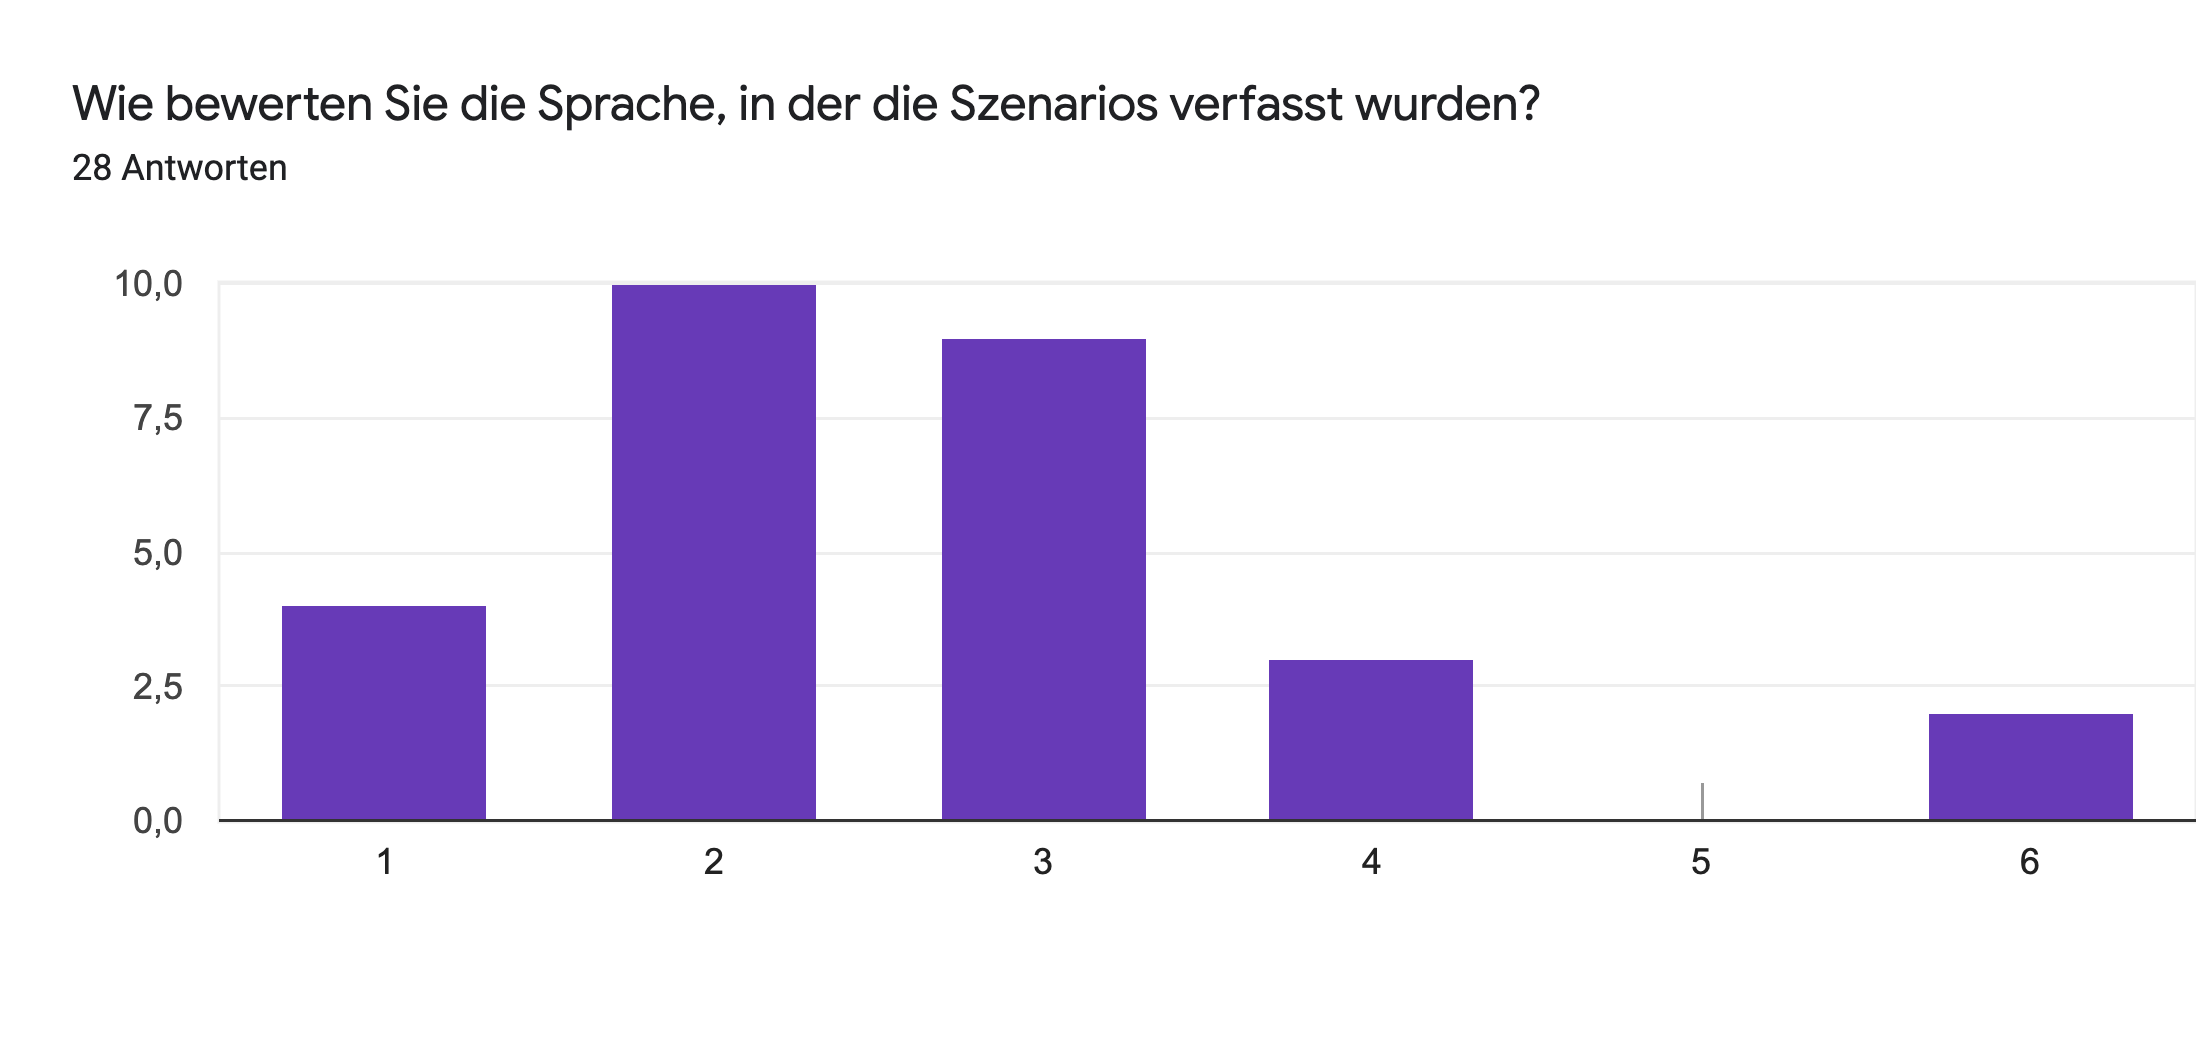
\includegraphics[width=\textwidth]{images/language.png}
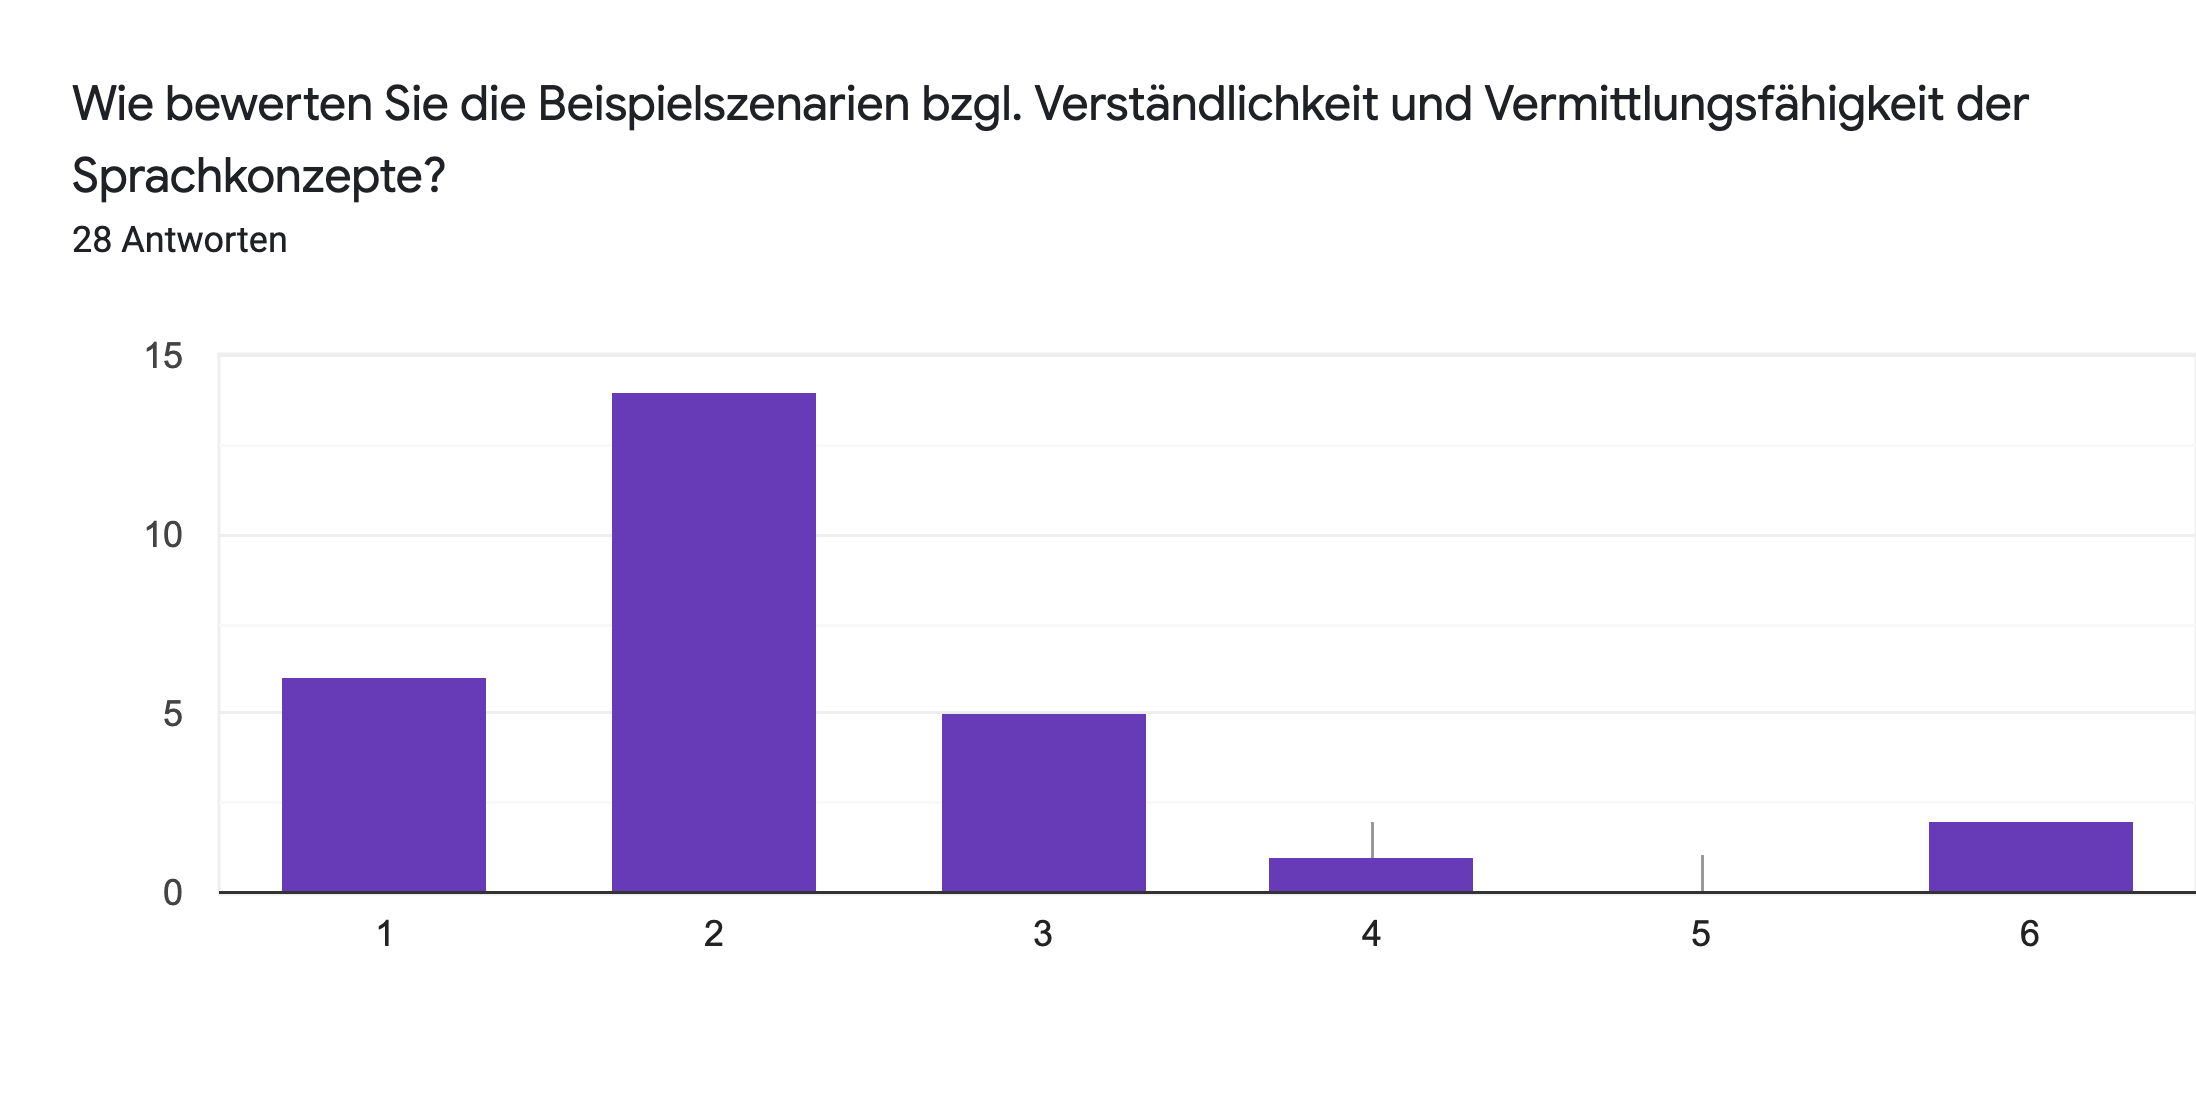
\includegraphics[width=\textwidth]{images/examples.png}
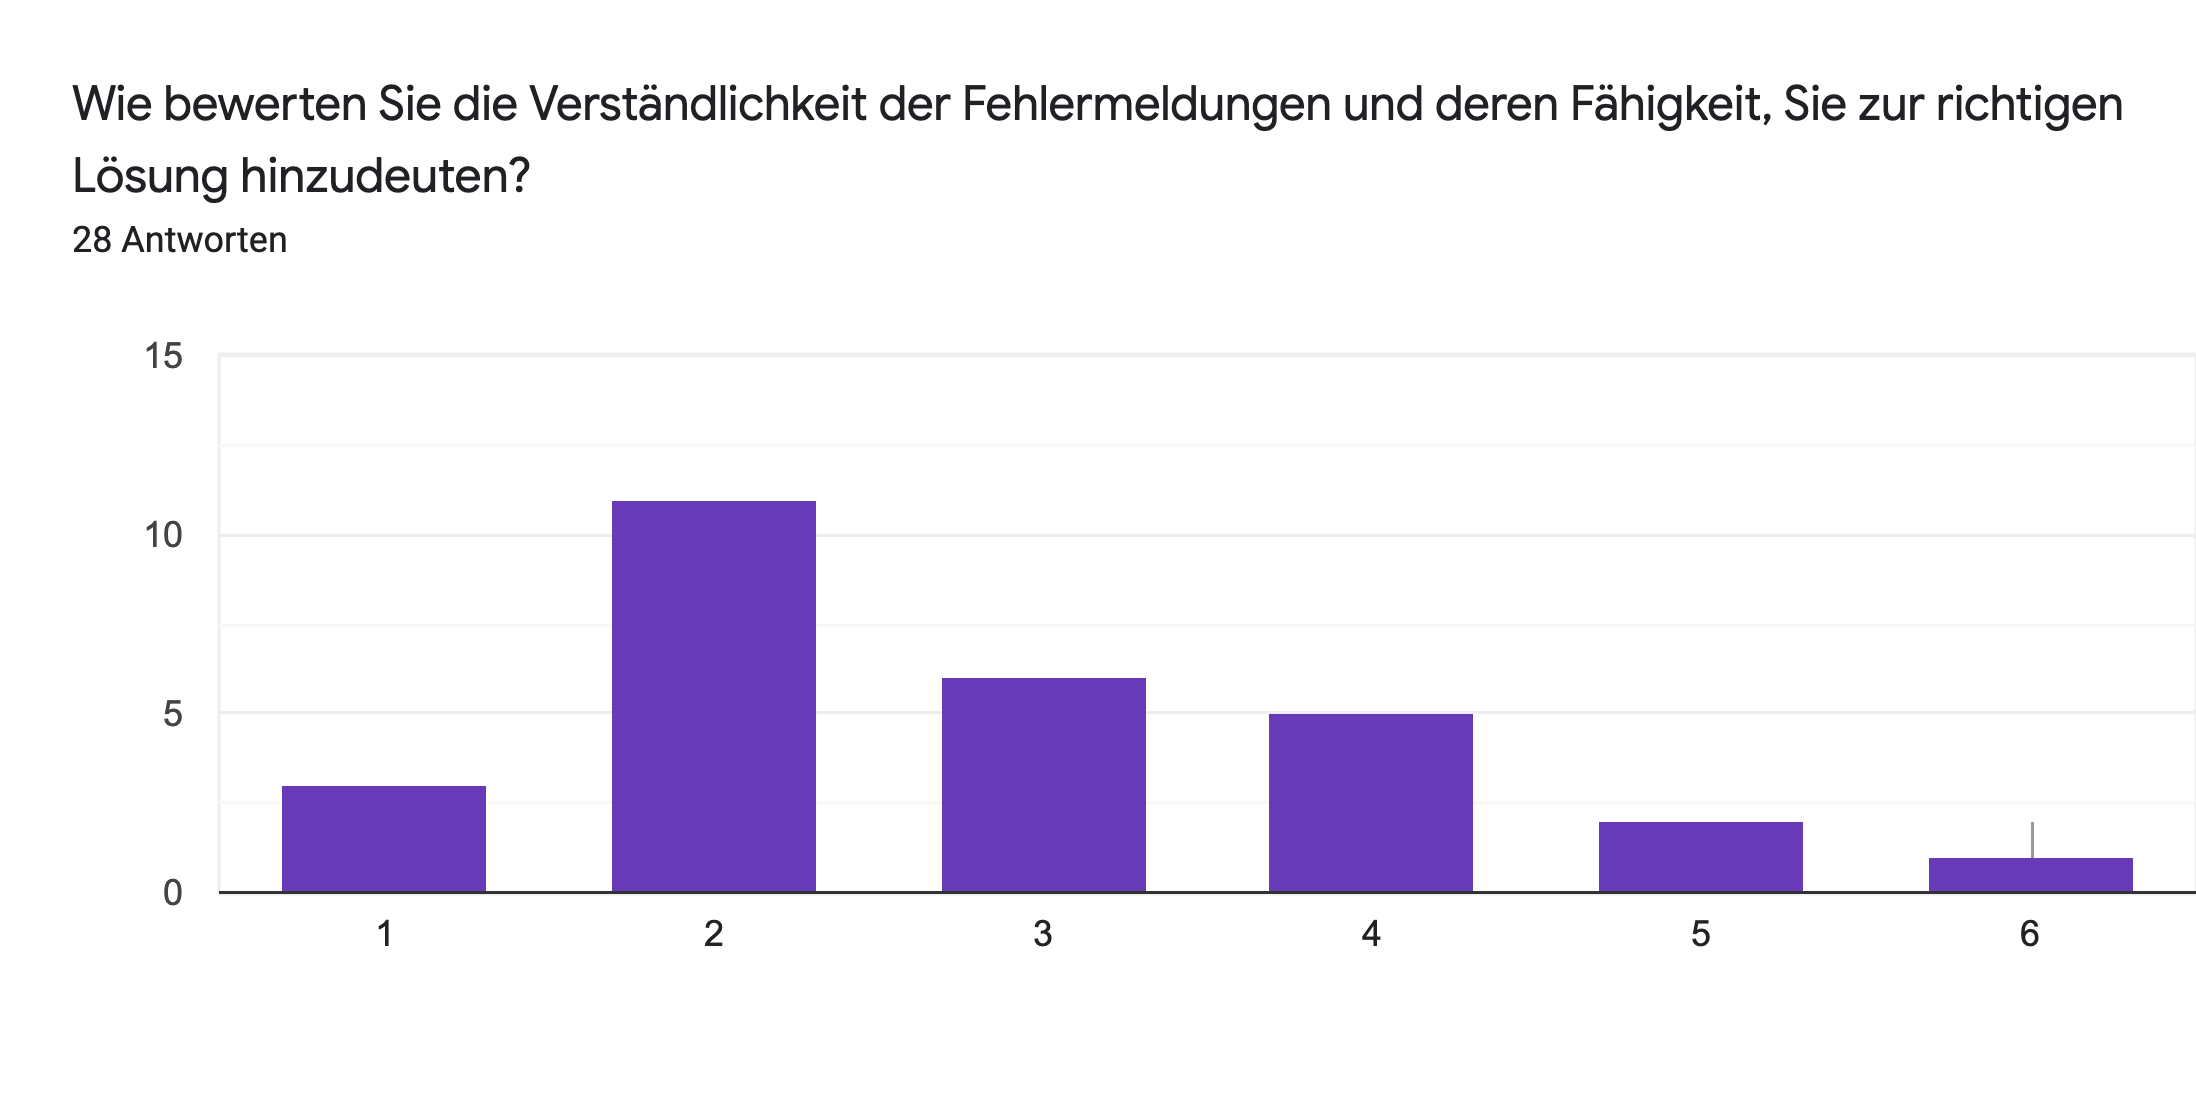
\includegraphics[width=\textwidth]{images/errors.png}
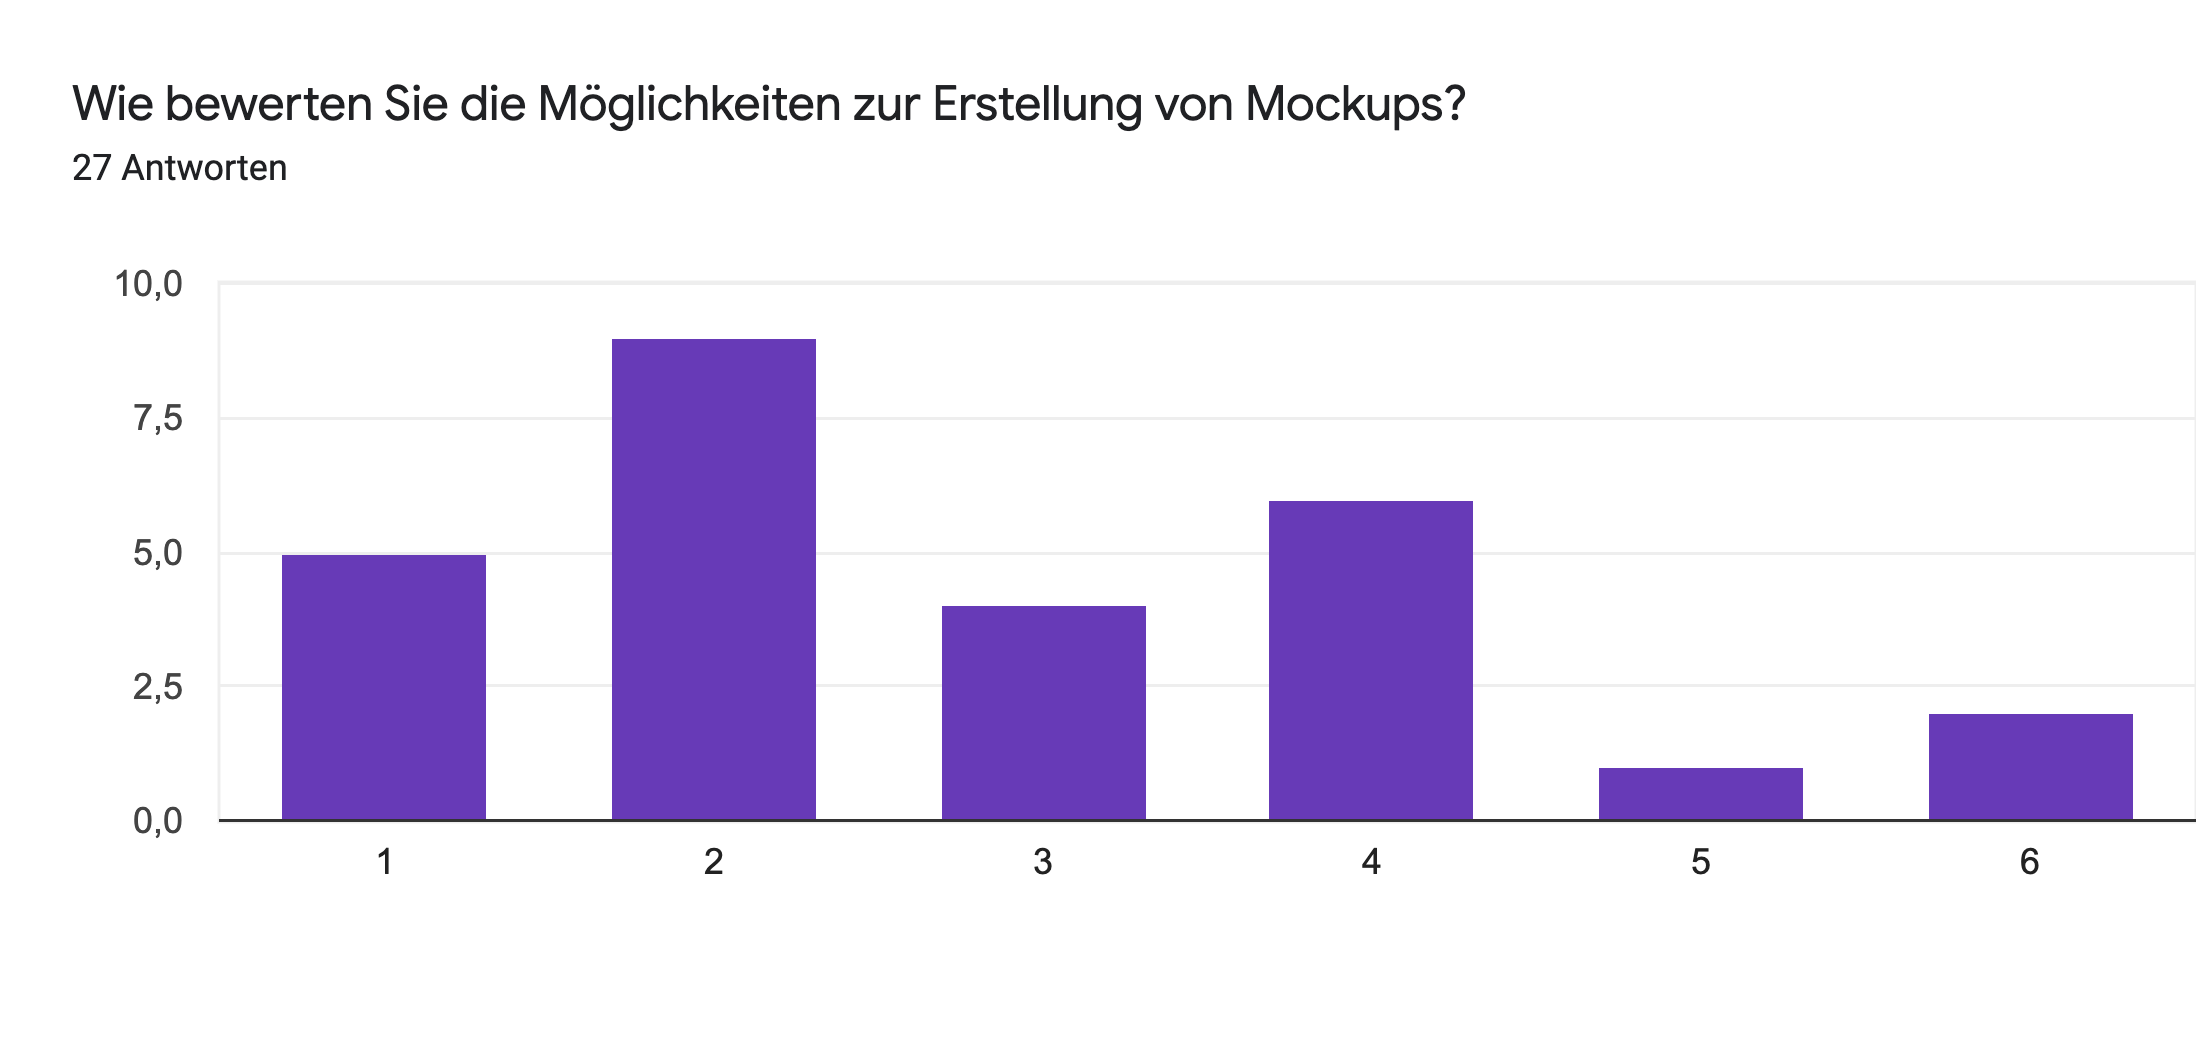
\includegraphics[width=\textwidth]{images/mockups.png}
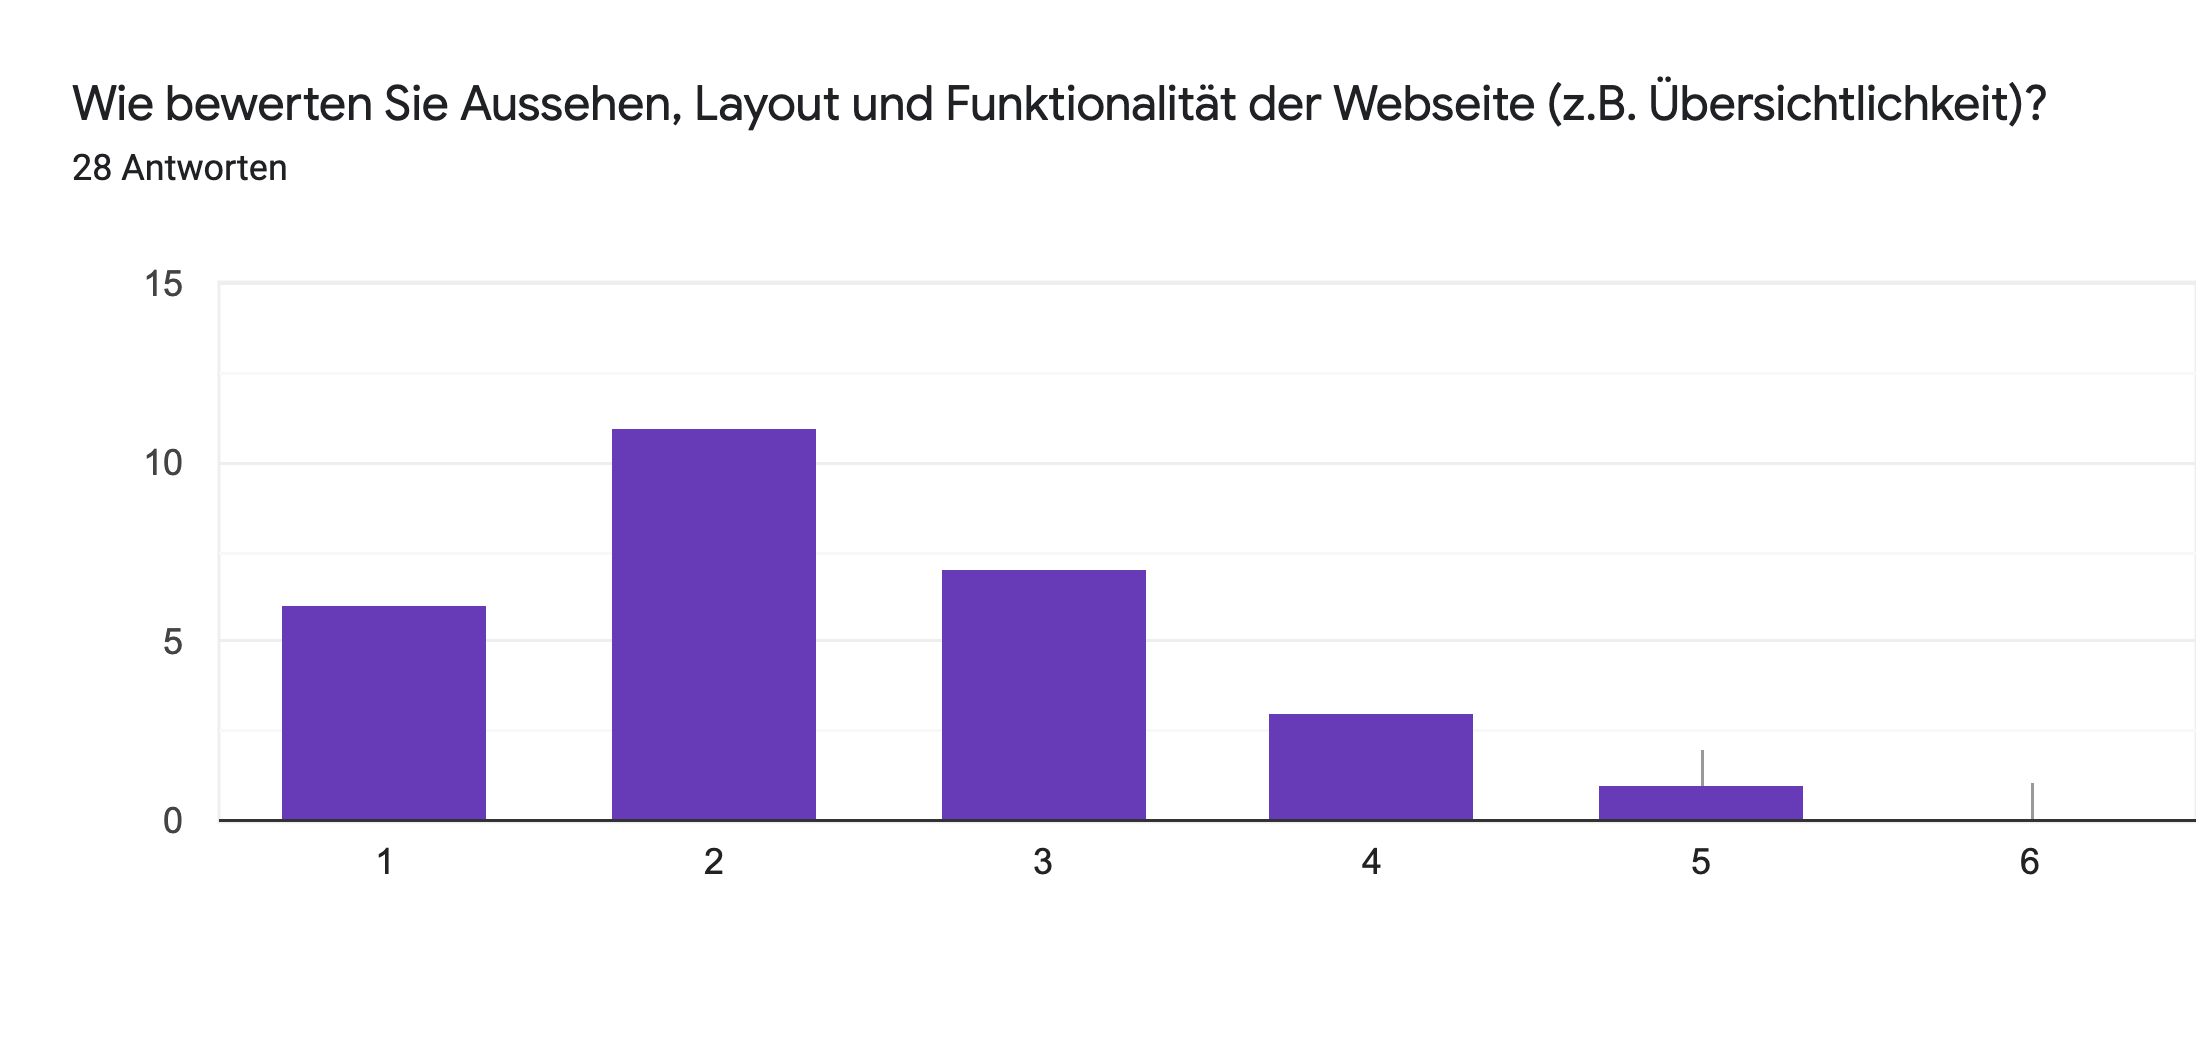
\includegraphics[width=\textwidth]{images/website.png}
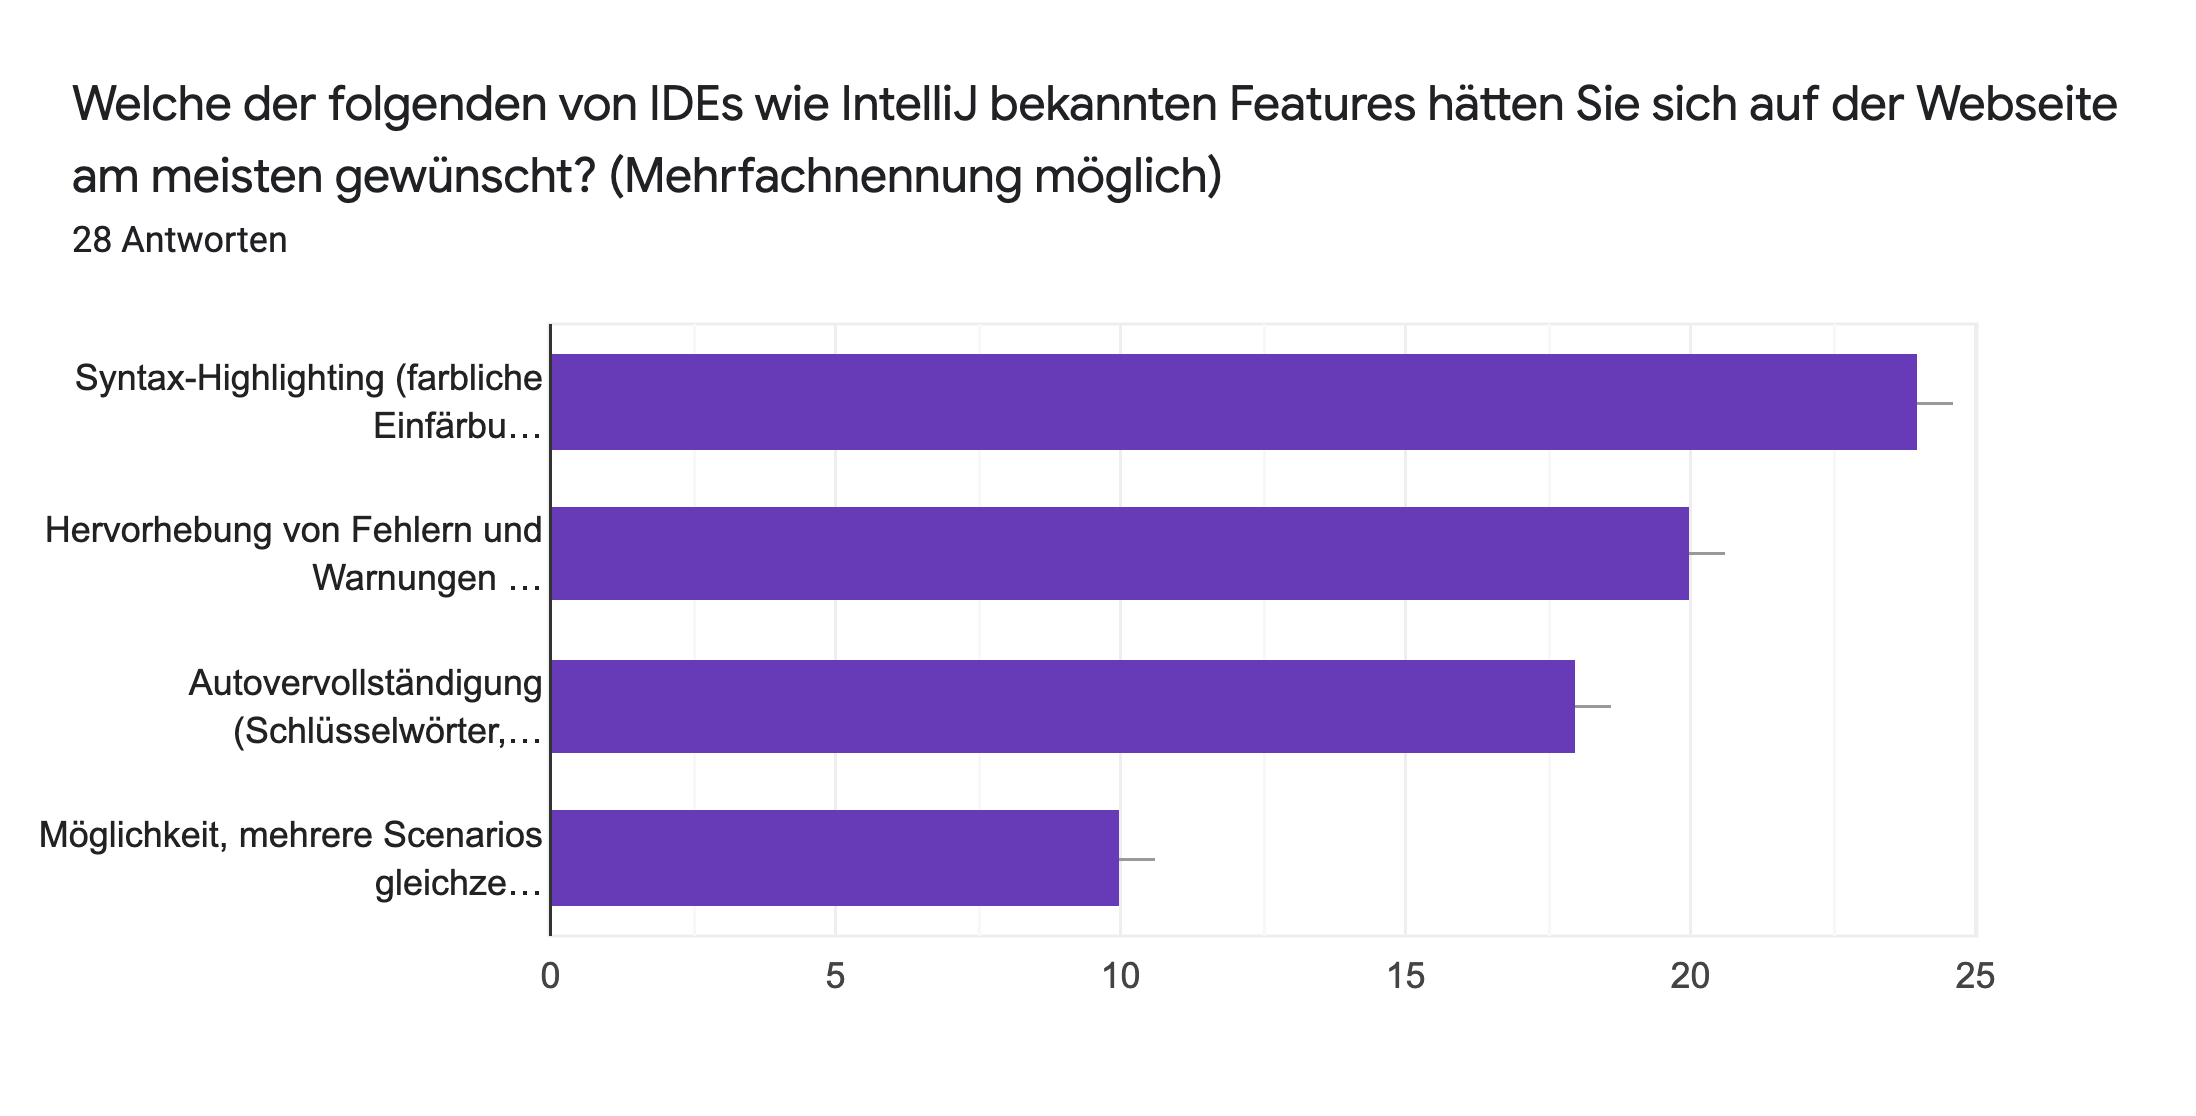
\includegraphics[width=\textwidth]{images/editor-features.png}

%Some guidelines and examples are given in the following.
%
%\section{Figures}
%
%A simple example of a figure can be found in \fig{fig:simple_figure}. A more complex figure including subfigures is show in \fig{fig:figure_with_subfigures}. Here each subfigure can be addressed separately (e.g., \fig{fig:subfigure1} and \fig{fig:subfigure2}). Please use vector graphics (pdf, eps obtained from svg, etc.) whenever possible. Pixel formats like jpeg, bmp, etc. should only be used for real photographs.
%
%\begin{figure}[!h]
%	\centering
%	\fbox{\parbox{5cm}{\centering ~\vspace{1.5cm}\\Dummy\\~\vspace{1.5cm}}} %replace this line by: \includegraphics{path to image}
%	\caption{Simple figure}
%	\label{fig:simple_figure}
%\end{figure}
%
%\begin{figure}[!h]
%	\centering
%	\begin{subfigure}[b]{7cm}
%		\centering
%		\fbox{\parbox{5cm}{\centering ~\vspace{1.5cm}\\Dummy\\~\vspace{1.5cm}}} %replace this line by: \includegraphics{path to image}
%		\caption{Caption of subfigure a (can be empty)}
%		\label{fig:subfigure1}
%	\end{subfigure}
%	\begin{subfigure}[b]{7cm}
%		\centering
%		\fbox{\parbox{5cm}{\centering ~\vspace{1.5cm}\\Dummy\\~\vspace{1.5cm}}} %replace this line by: \includegraphics{path to image}
%		\caption{Caption of subfigure b (can be empty)}
%		\label{fig:subfigure2}
%	\end{subfigure}
%	\caption{Figure using subfigures}
%	\label{fig:figure_with_subfigures}
%\end{figure}
%
%
%\section{Tables}
%
%Examples of tables can be found in \tab{tab:simple_table} and \tab{tab:complex_table}. In general vertical lines are not necessary and should be avoided (see \cite{Fear05} for more about table styles).
%
%\begin{table}[!h]
%	\renewcommand{\arraystretch}{1.1}
%	\caption{A very simple table}
%	\label{tab:simple_table}
%	\centering
%	\begin{tabular}{cccc}
%		\toprule
%		& Apple & Orange & Banana \\
%		\midrule
%		Colour       & green & orange & yellow\\
%		\bottomrule
%	\end{tabular}
%\end{table}
%
%\begin{table}[!h]
%	\renewcommand{\arraystretch}{1.1}
%	\caption{An example of a more complex table}
%	\label{tab:complex_table}
%	\centering
%	\begin{tabular}{ccC{1cm}C{1cm}C{1cm}C{1cm}C{1cm}C{1cm}C{1cm}C{1cm}C{1cm}C{1cm}C{1cm}}
%		\toprule
%		& & \multicolumn{4}{c}{RPAG algorithm} & \multicolumn{5}{c}{RPAGT (proposed)}\\
%		\cmidrule(rl){3-6} \cmidrule(rl){7-11}
%		$N$ & $N_\text{uq}$ & S & add ops & pure reg. & reg. ops & S & add ops & pure reg. & reg. ops & impr.\\
%		\cmidrule(rl){1-11}
%		6   & 3  & 3 & 8  & 1 & 9  & 2 & 5  & 0 & 5  & 44.4\% \\
%		10  & 5  & 3 & 10 & 3 & 13 & 2 & 6  & 2 & 8  & 38.5\% \\
%		13  & 7  & 3 & 14 & 2 & 16 & 2 & 8  & 2 & 10 & 37.5\% \\
%		20  & 10 & 3 & 15 & 4 & 18 & 2 & 9  & 3 & 12 & 33.3\% \\
%		28  & 14 & 3 & 20 & 3 & 23 & 2 & 15 & 2 & 17 & 26.1\% \\
%		41  & 21 & 3 & 31 & 1 & 32 & 2 & 23 & 2 & 25 & 21.9\% \\
%		61  & 31 & 3 & 39 & 3 & 42 & 2 & 32 & 2 & 34 & 19.0\% \\
%		119 & 54 & 3 & 62 & 7 & 69 & 2 & 56 & 1 & 57 & 17.4\% \\
%		151 & 71 & 3 & 79 & 4 & 83 & 2 & 72 & 2 & 74 & 10.8\% \\
%		\cmidrule(rl){1-11}
%		avg.: & 24 & & 30.89 & 3.56 & 33.89 & & 25.11 & 1.78 & 26.89 & 27.7\% \\
%		\bottomrule
%	\end{tabular}
%\end{table}
